State-of-the-art LLMs continue to struggle with factual errors~\citep{mallen2022not,min2023factscore} despite their increased model and data scale~\citep{ouyang2022training}. 
Retrieval-Augmented Generation (RAG) methods (Figure~\ref{fig:taxonomy} left;~\citealt{lewis2020retrieval,guu2020retrieval}) augment the input of LLMs with relevant retrieved passages,  reducing factual errors in knowledge-intensive tasks~\citep{ram2023context, asai-etal-2023-retrieval}. 
However, these methods may hinder the versatility of LLMs or introduce unnecessary or off-topic passages that lead to low-quality generations ~\citep{pmlr-v202-shi23a} since they retrieve passages indiscriminately regardless of whether the factual grounding is helpful.
Moreover, the output is not guaranteed to be consistent with retrieved relevant passages~\citep{gao2023enabling} since the models are not explicitly trained to leverage and follow facts from provided passages. 
This work introduces {\bf Self-Reflective Retrieval-augmented Generation (\model)} to improve an LLM's generation quality, including its factual accuracy without hurting its versatility, via on-demand retrieval and self-reflection. 
We train an arbitrary LM in an end-to-end manner to learn to reflect on its own generation process given a task input by generating both task output and intermittent special tokens (i.e., \textit{reflection tokens}). Reflection tokens are categorized into \textit{retrieval} and \textit{critique} tokens to indicate the need for retrieval and its generation quality respectively (Figure~\ref{fig:taxonomy} right). 
{
In particular, given an input prompt and preceding generations, \model first determines if augmenting the continued generation with retrieved passages would be helpful. If so, 
it outputs a {\bf retrieval} token that calls a retriever model on demand (Step 1). 
Subsequently, \model concurrently processes multiple retrieved passages, evaluating their relevance and then {\bf generating} corresponding task outputs (Step 2). It then generates critique tokens to \textbf{criticize} its own output and choose best one (Step 3) in terms of factuality and overall quality. 
This process differs from conventional RAG (Figure~\ref{fig:taxonomy} left), which consistently retrieves a fixed number of documents for generation regardless of the retrieval necessity (e.g., the bottom figure example does not require factual knowledge) and never second visits the generation quality.
Moreover, \model provides citations for each segment with its self-assessment of whether the output is supported by the passage, leading to easier fact verification. }

\model trains an arbitrary LM to generate text with reflection tokens by unifying them as the next token prediction from the expanded model vocabulary. 
{
We train our generator LM on a diverse collection of text interleaved with reflection tokens and retrieved passages. 
%\sandy{Should the following info be in the Abstract, too, as a benefit of your framework?}
Reflection tokens, inspired by reward models used in reinforcement learning~\citep{ziegler2019fine, ouyang2022training}, are inserted offline into the original corpus by a trained {\it critic} model. This eliminates the need to host a critic model during training, reducing overhead.
The critic model, in part, is supervised on a dataset of input, output, and corresponding reflection tokens collected by prompting a propriety LM (i.e., GPT-4; \citealt{openai2023gpt}).
While we draw inspiration from studies that use control tokens 
to start and guide text generation~\citep{lu2022quark,keskar2019ctrl},
our trained LM uses critique tokens to assess its own predictions after each generated segment as an integral part of the generation output.
}


{\model further enables a customizable 
decoding algorithm to satisfy hard or soft constraints, which are defined by reflection token predictions.}
In particular, our inference-time algorithm enables us to (1) flexibly adjust retrieval frequency for different downstream applications and (2) customize models' behaviors to user preferences by leveraging reflection tokens through segment-level beam search using the weighted linear sum of the reflection token probabilities as segment score. 


\begin{figure}[t!]
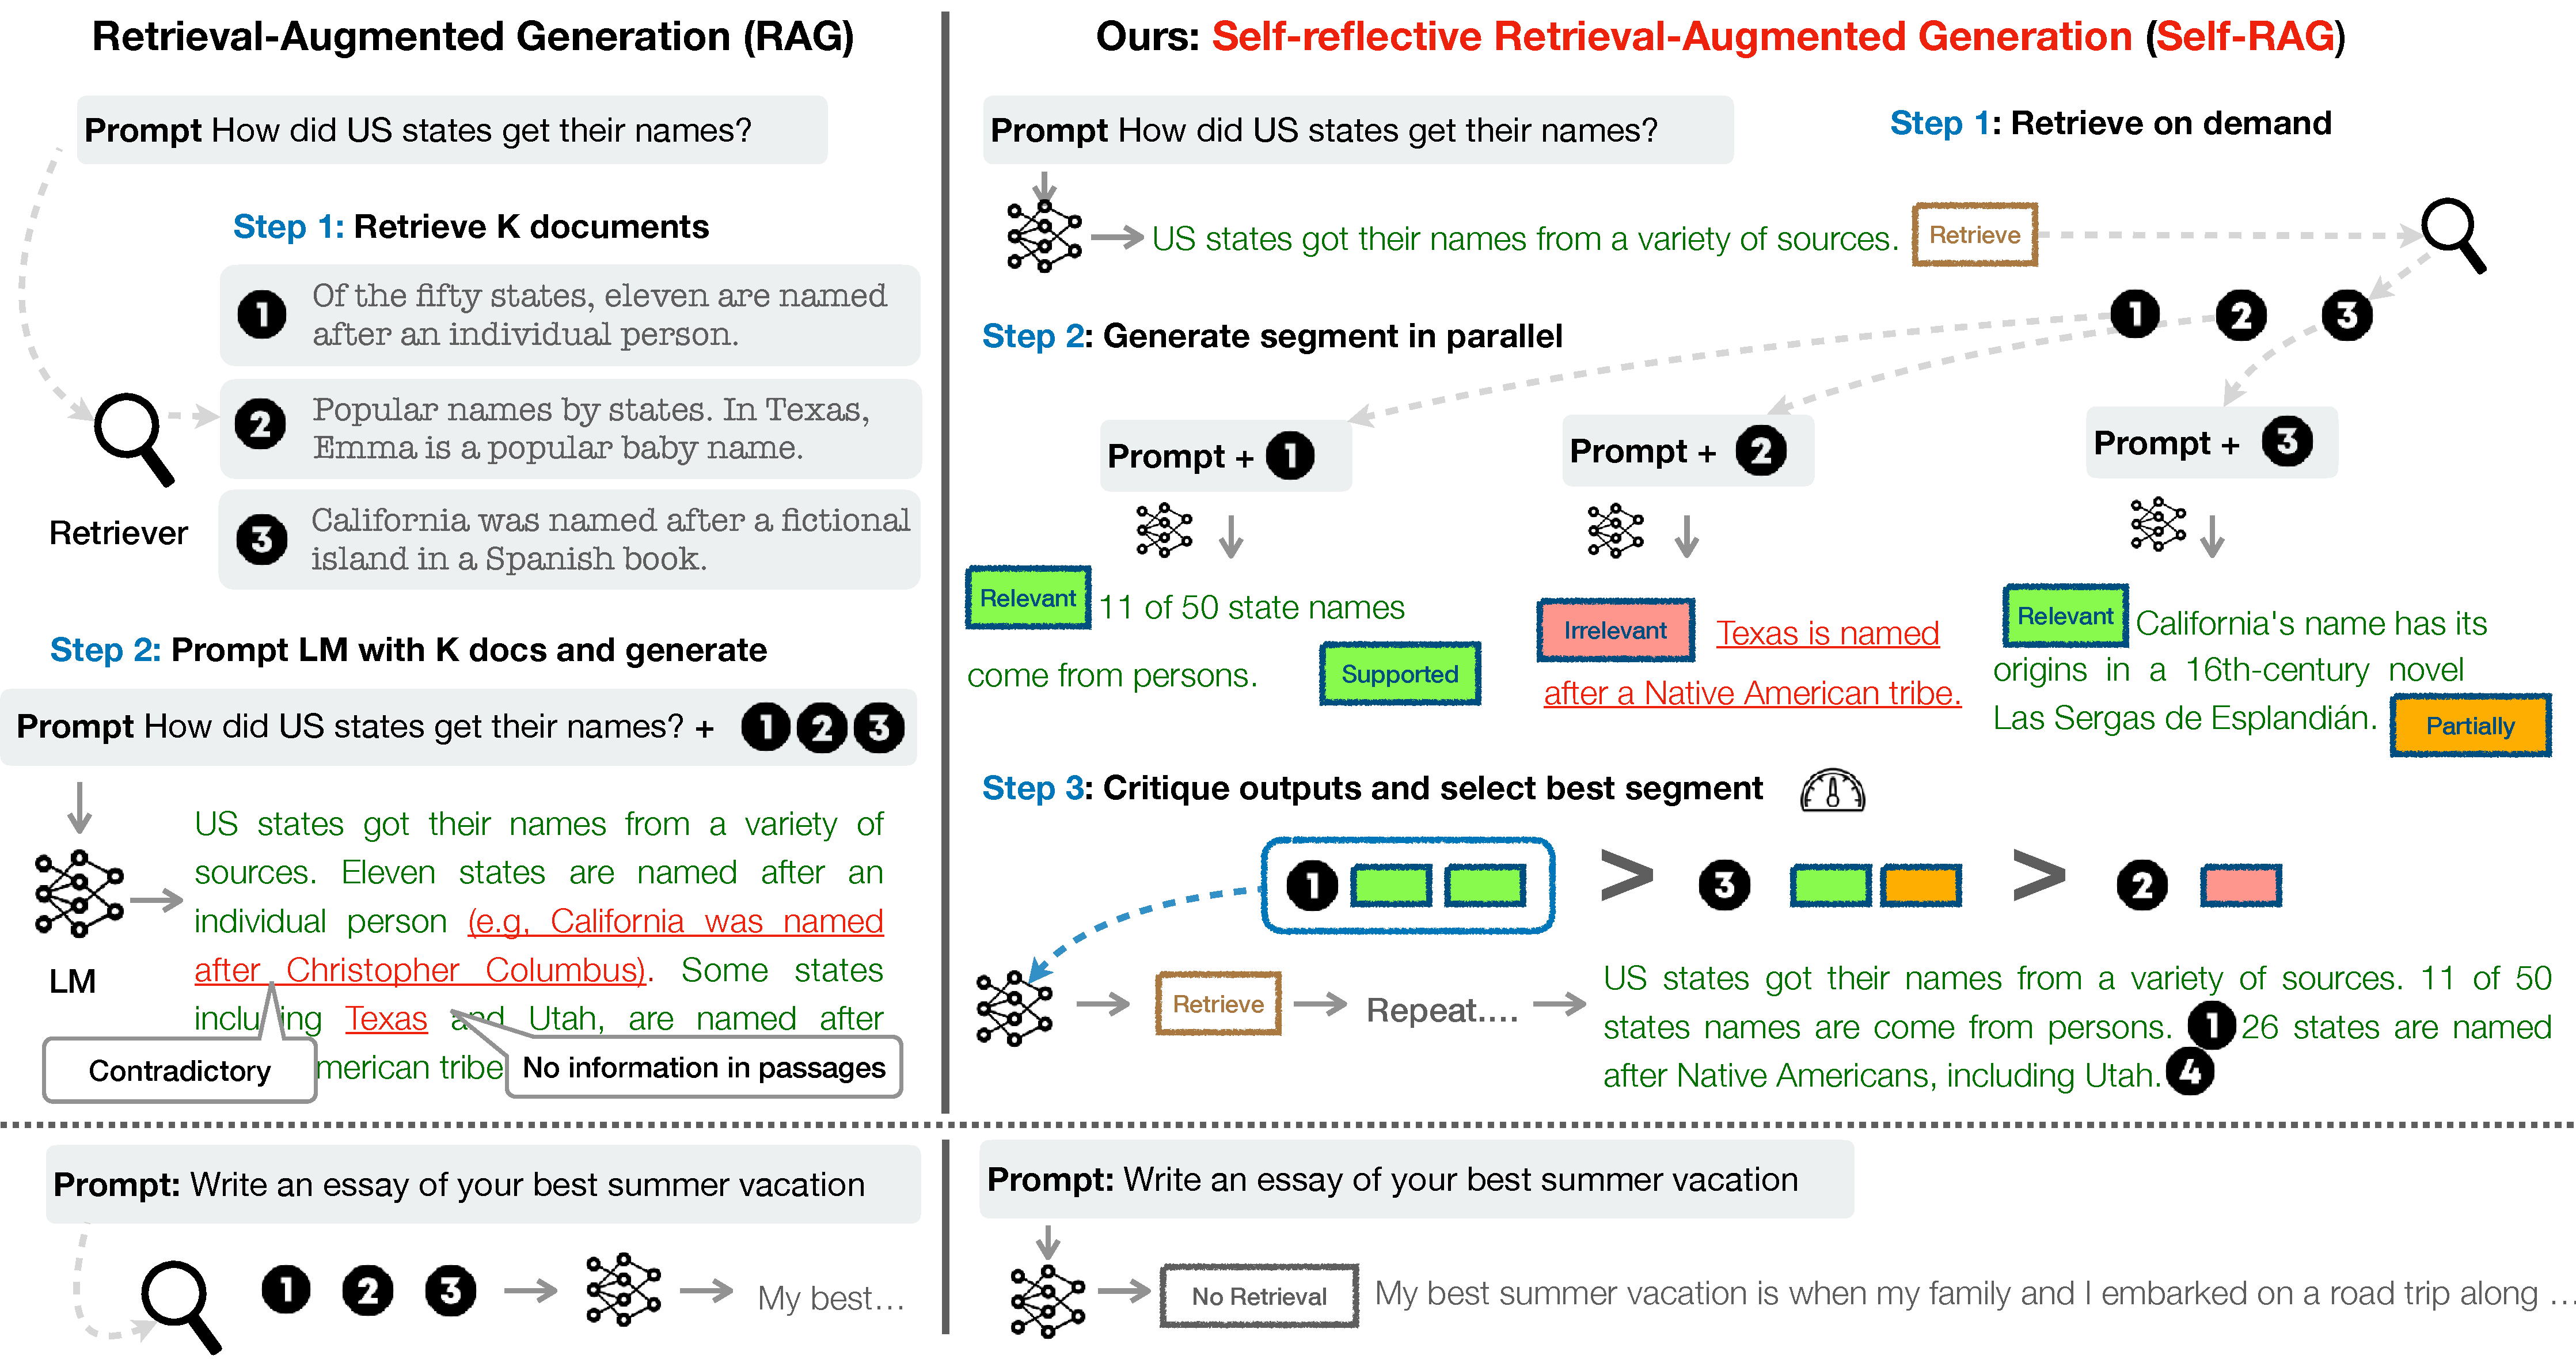
\includegraphics[width=\textwidth]{figs/teaser_self_rag_v8.pdf}\caption{Overview of \model. \model learns to retrieve, critique, and generate text passages to enhance overall generation quality, factuality, and verifiability. 
} \label{fig:taxonomy}
\end{figure}

Empirical results on six tasks, including reasoning and long-form generation, demonstrate that \model significantly outperforms pre-trained and instruction-tuned LLMs that have more parameters and  widely adopted RAG approaches with higher citation accuracy. 
In particular, \model outperforms retrieval-augmented ChatGPT on four tasks, Llama2-chat~\citep{touvron2023llama} and Alpaca~\citep{dubois2023alpacafarm} on all tasks. 
Our analysis demonstrates the effectiveness of training and inference with reflection tokens for overall performance improvements as well as test-time model customizations (e.g., balancing the trade-off between citation previsions and completeness). 
